\section{Thiết kế trực quan hóa}

\subsection{Nguyên tắc trực quan áp dụng}

Các figure được thiết kế theo các nguyên tắc:
\begin{itemize}[leftmargin=1.2cm]
    \item \textbf{Đúng nhiệm vụ phân tích:} line chart cho xu hướng theo $n$, bar chart cho so sánh snapshot tại $n$ lớn nhất.
    \item \textbf{Nhất quán thị giác:} giữ nguyên màu và marker giữa các figure.
    \item \textbf{Đọc được khi in:} độ tương phản cao, marker phân biệt rõ, lưới phụ ở mức vừa đủ.
    \item \textbf{Không gây hiểu nhầm scale:} ghi rõ linear hay log scale ngay trong tiêu đề/trục.
\end{itemize}

\subsection{Danh mục figure chính}

\begin{table}[H]
\centering
\renewcommand{\arraystretch}{1.2}
\begin{tabular}{p{4.3cm}p{2.6cm}p{6.8cm}}
\toprule
\textbf{Figure} & \textbf{Scale} & \textbf{Mục đích} \\
\midrule
\texttt{figure\_01\_time\_linear} & Linear-$y$ & Thể hiện mức chênh lệch tuyệt đối thời gian chạy. \\
\texttt{figure\_02\_time\_logy} & Log-$y$ & Làm rõ xu hướng tăng và khác biệt tốc độ tăng giữa thuật toán. \\
\texttt{figure\_03\_time\_bar\_nmax\_logy} & Log-$y$ & So sánh trực tiếp ba thuật toán tại $n$ lớn nhất theo từng kiểu dữ liệu. \\
\texttt{figure\_04\_comparisons\_loglog} & Log-log & Quan sát số phép so sánh (phân tích phụ trợ). \\
\bottomrule
\end{tabular}
\caption{Bộ figure được dùng trong báo cáo}
\label{tab:figure-catalog}
\end{table}

\subsection{Hình minh họa chính}

\begin{figure}[H]
    \centering
    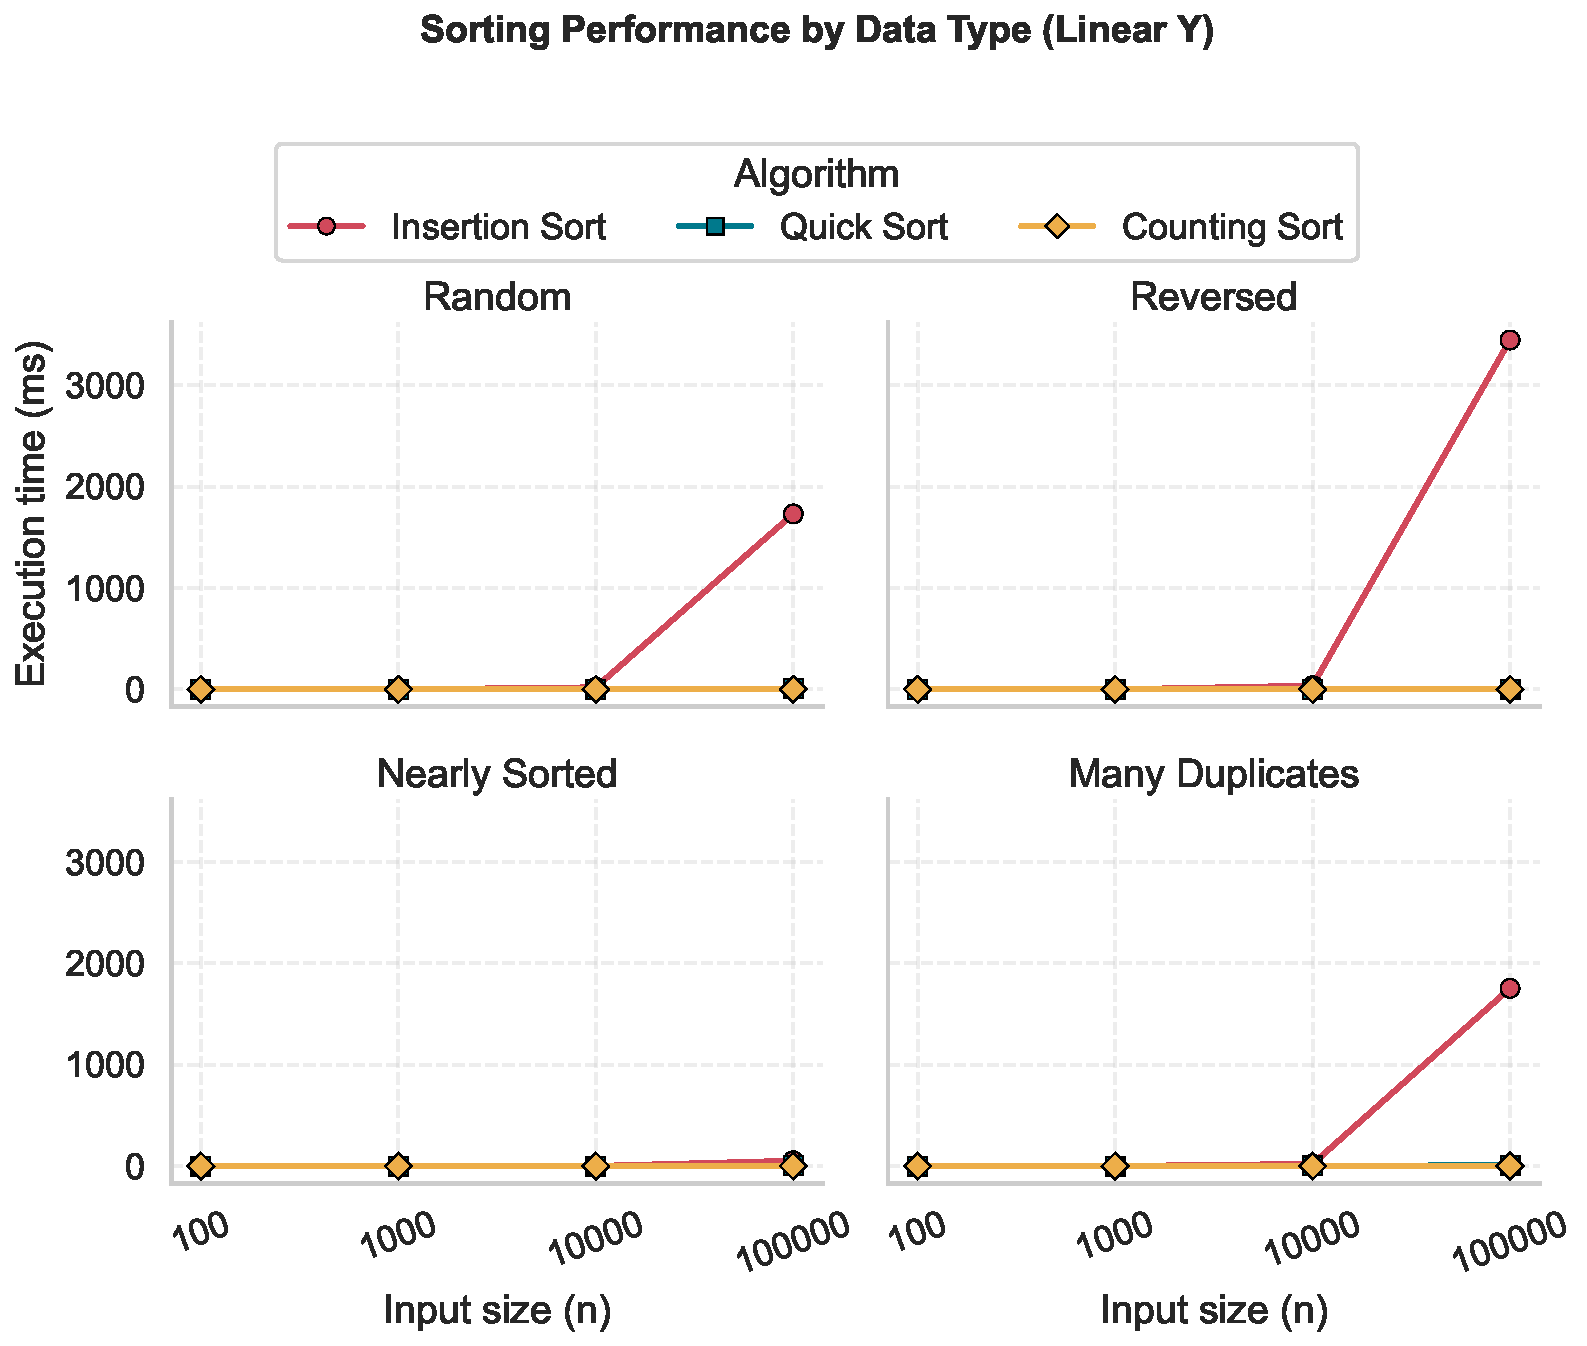
\includegraphics[width=0.98\textwidth]{../figures/figure_01_time_linear.pdf}
    \caption{Hiệu năng sắp xếp theo từng kiểu dữ liệu với trục $y$ tuyến tính.}
    \label{fig:time-linear}
\end{figure}

\begin{figure}[H]
    \centering
    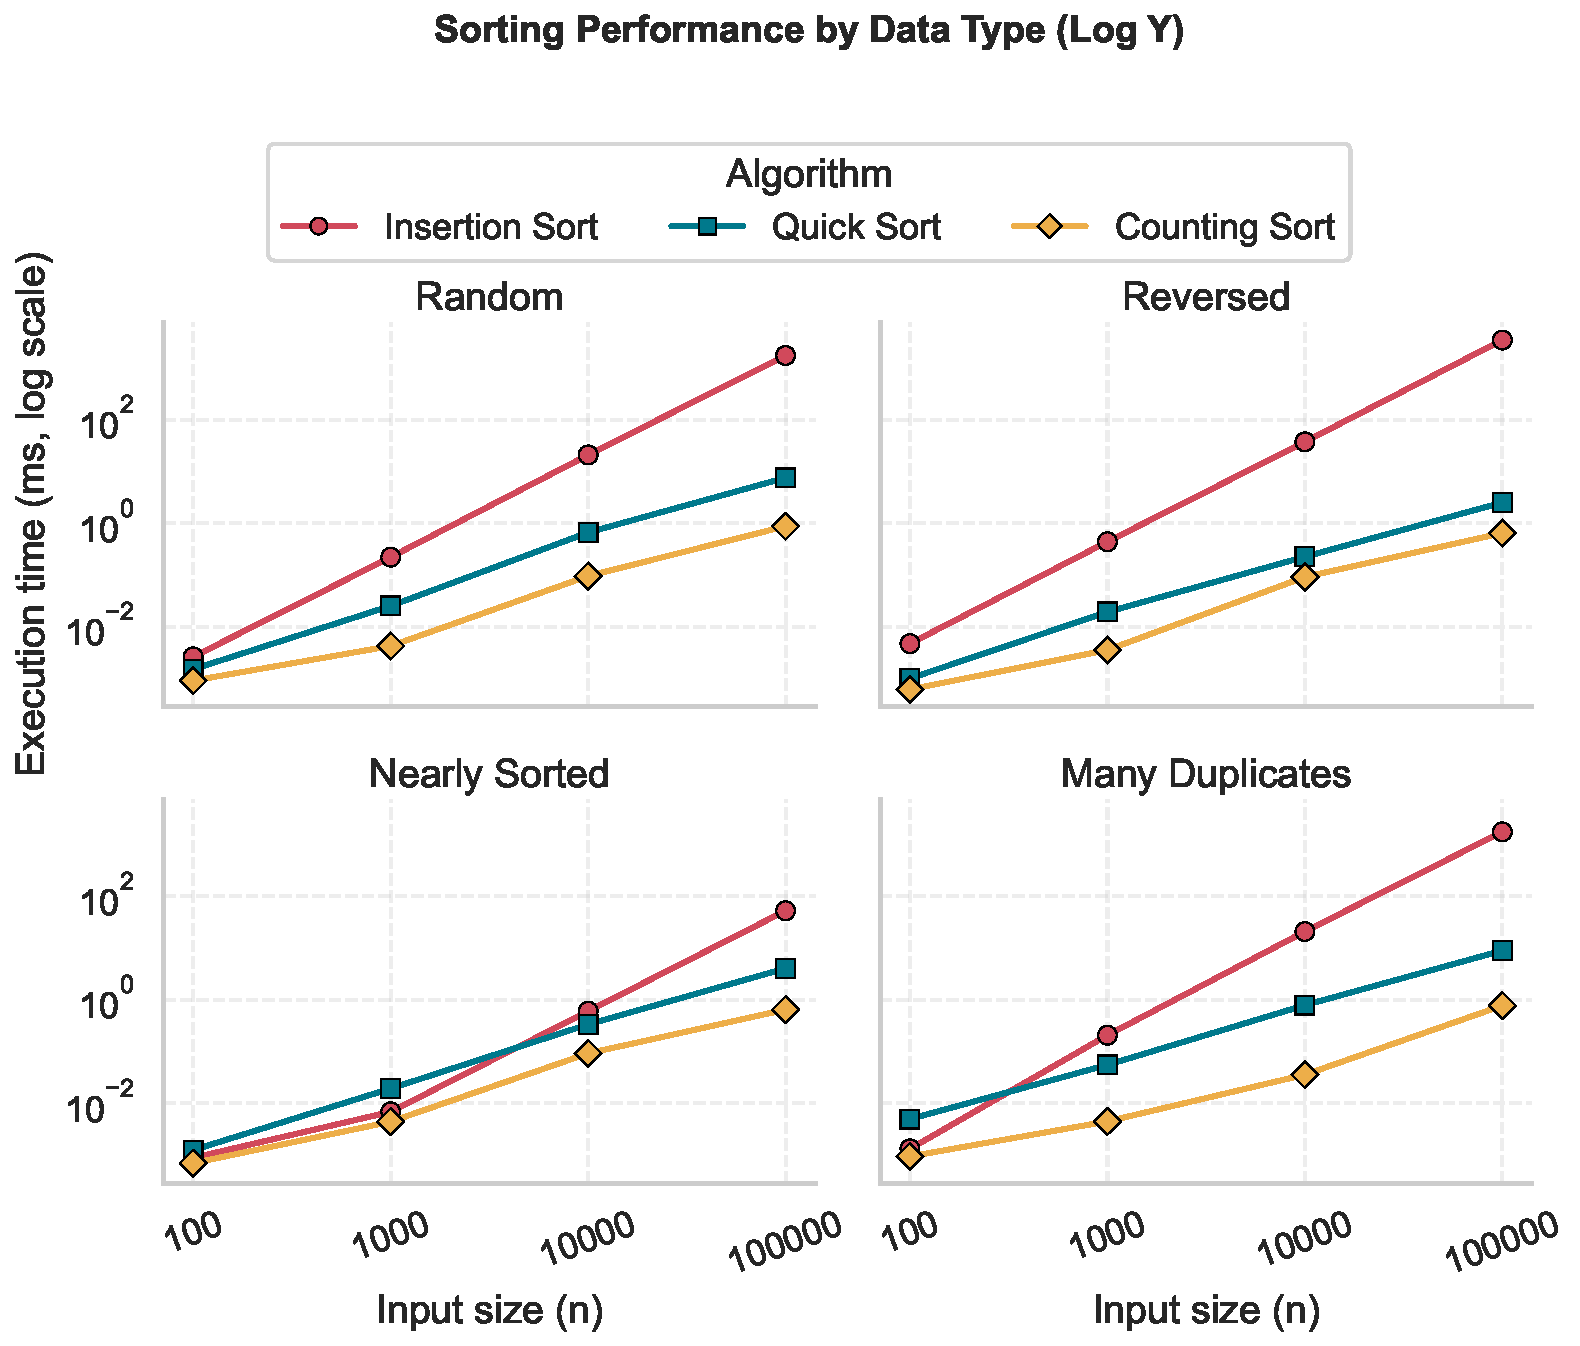
\includegraphics[width=0.98\textwidth]{../figures/figure_02_time_logy.pdf}
    \caption{Hiệu năng sắp xếp theo từng kiểu dữ liệu với trục $y$ log.}
    \label{fig:time-logy}
\end{figure}

\begin{figure}[H]
    \centering
    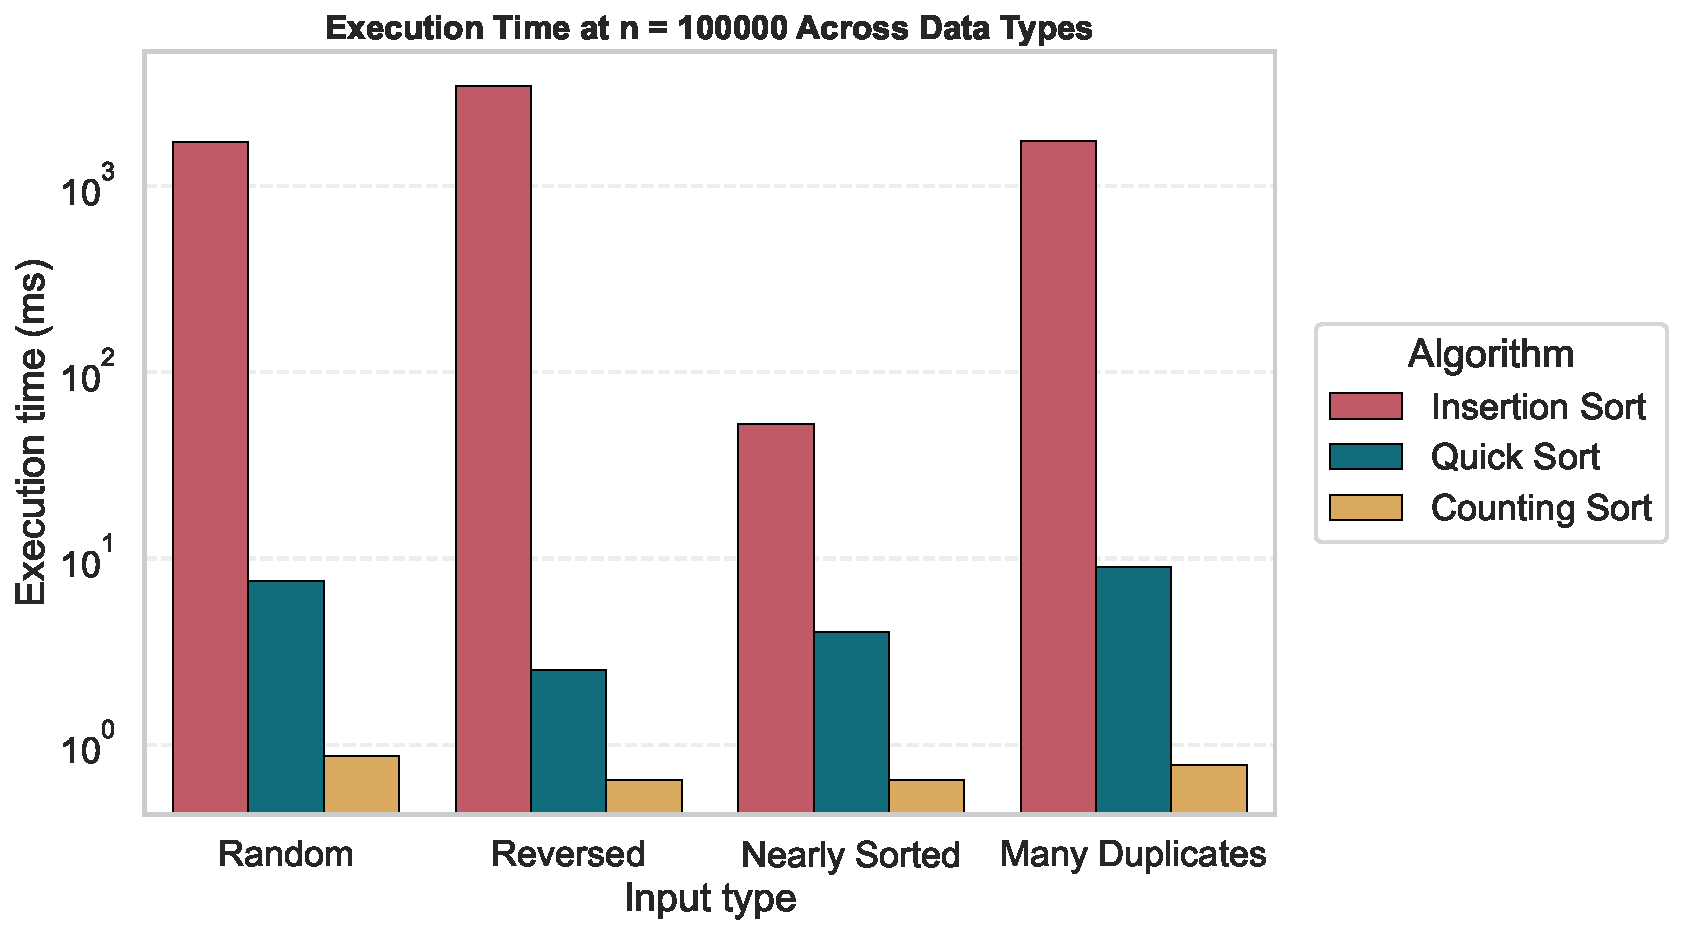
\includegraphics[width=0.95\textwidth]{../figures/figure_03_time_bar_nmax_logy.pdf}
    \caption{So sánh thời gian chạy tại $n=100000$ giữa các kiểu dữ liệu.}
    \label{fig:bar-nmax}
\end{figure}

\begin{figure}[H]
    \centering
    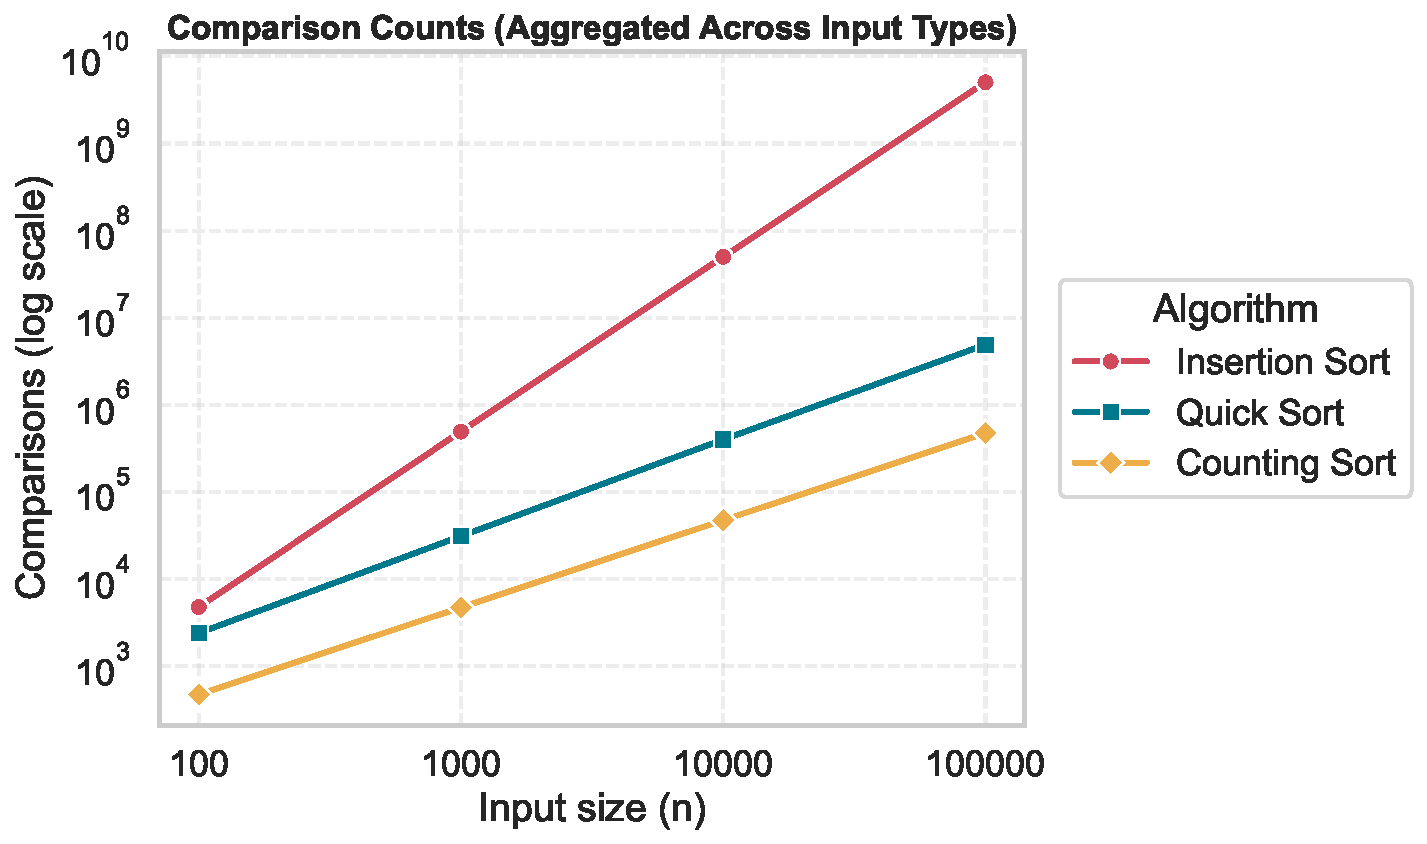
\includegraphics[width=0.95\textwidth]{../figures/figure_04_comparisons_loglog.pdf}
    \caption{Biểu đồ phụ trợ số phép so sánh trên thang log-log.}
    \label{fig:comparisons}
\end{figure}
